    \documentclass[11pt]{article}
    %	options include 12pt or 11pt or 10pt
    %	classes include article, report, book, letter, thesis
    
    \title{HW10}
    \author{Shane Drafahl}
    \date{16 October ,2017}
    \usepackage{graphicx}
    \usepackage{epstopdf}
    \usepackage{graphics}

    \begin{document}
    \maketitle

     1. For union for $ L_{1} $ and $ L_{2} $ I have machines $ M_{1} $ and $ M_{2} $. Given 
     an input $ x \in L_{1} \cup L_{2} $ I give x to $ M_{1} $ and $ M_{2} $ and if its accepted by
     either machine that means they are accepted. Similar to intersection but both machines must be accepted.
     I would build this turring machine by getting two tape and with input x and then dove tailing the 
     two tape into each relative turring machine. For example below is a representation of the tape
     where $ b_{1} = a_{1} $ and so on and so forth.



    \begin{figure}[!htb]
        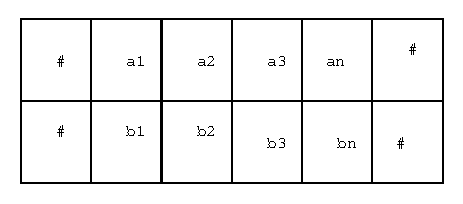
\includegraphics[scale=.7]{./turring.eps}
    \end{figure}

    $ \newline $

    For reversal I would simply copy the input from one side of the tape to the other in reverse
    order. I would then have the same turring machine dove tail both peices of tape and if both are 
    accepted then the whole thing is accepted.

    $ \newline $

    2. Given a string that z = xy and you have $ M_{1} $, $ M_{2} $. You create every possible combination
    of ways to divided up z onto multiple peices of tape. For example if x = ab and y = cd then
    you have 
    $ \newline $
    $ T[a]_{1} ...  T[bcd]^{2} $ 
    $ \newline $
    $ T[ab]_{3} ... T[cd]_{4} $
    $ \newline $
    $  T[abc]_{5} ... T[d]_{6} $
    $ \newline $
    Where $ T[]_{n} $ is a peice of tape. $ M_{1} $ dove tails for every odd indexed tape and $ M_{2} $
    does every even. If both of the machines have at least one accepting string then the whole thing is
    accepted. 


    $ \newline $

    3. a 

    $ \newline $

    For this turring machine it would depend on if it goes left,right, or does nothing
    $ \newline $
    $ \delta (a_{n}, a_{n}) $ = $ (a_{n + 1}, R) $ and push  (GO RIGHT)
    $ \newline $
    $ \delta (a_{n}, a_{n}) $ = $ (a_{n - 1}, L) $ (GO LEFT)
    $ \newline $
    $ \delta (a_{n}, a_{n}) $ = $ (a_{n}, a_{n}) $ (Do Nothing)
    $ \newline $
    b. 
    $ \newline $
    
    To prove that all languages accepted by PA's can be accepted by M we will prove that the accepted
    languages of $ PA \subset M $. We can prove this because we can simulate a PA with M by starting
    the head on the left most data on the read only tape and only using $ \Gamma_{1} $ and reading
    from left to right.  

    $ \newline $

    We can prove that it is equivalant to a turring machine because $ M \subset T $ and $ T \subset M $.
    In this case we can prove $ M \subset T $ because a Turring machine can use two peices of tape to
    simulate the two stacks and a third as the read only tape. We can also prove $ T \subset M $.
    We can simulate a turring machine because we can put all the contents left of the head in $ \Gamma_{1} $.
    and to the right $ \Gamma_{2} $. If we want to move right we pop $ \Gamma_{2} $ and left $ \Gamma_{1} $.
    Therfore they are equal. We also know that all languages accepted by any type of PA including
    NPDA or determinsitic ones can also be accepted by a turring machine so that is another reason 
    M can accept the same languages as a class of automata.

    



    \end{document}